The results of the model independent limits are interpreted in terms of limits
on the fundamental Plank scale in $4 + n$ dimensions (M$_\mathrm{\, D}$) in the
\gls{led} scenario proposed by \gls{add}~\cite{ADDPaper}. In this model, a
number of compact extra dimensions, where only the graviton field is allowed to
propagate, are added to the usual 4 (three spatial dimensions and time) thus
effectively reducing the strength of the gravitational interaction whose scale,
M$_\mathrm{\, D}$, could be at the TeV scale. Figure~\ref{fig:add_observed} show
the expected and observed limits at 95\% CL on M$_\mathrm{\, D}$ as a function
of the large extra dimensions $n$. The dashed blue line shows the expected
limits using $36.1~\ifb$ with the $\pm 1 \sigma$ and $\pm 2 \sigma$ error bands
(green and yellow band respectively). The black solid line is the observed
limit. The previous results obtained with $3.2~\ifb$ are also reported for
comparison. In \cref{tab:add_limits} the limits where a
M$^4_\mathrm{\, D} / \hat{s}^2$ weighting factor (see
\cref{sec:valid-effect-field}) is applied to the visible cross section for
events with $\hat{s} > $ M$^2_\mathrm{\, D}$ (soft damping) where $\hat{s}$ is
the center of mass energy of the interacting partons is also reported in
parentheses; the effect of the the truncation is only noticeable in the ADD n =
6 model meaning that the analysis is probing values of M$_\mathrm{\, D}$ where
the effective theory can be trusted.

Values of M$_\mathrm{\, D}$ up to 7.7~TeV for n = 2 dimensions and 4.8~TeV for n
= 6 dimensions are excluded at 95\%~CL improving previous results.
\begin{table}[!hb]
  \centering
  \begin{tabular}{lcc}
    \toprule
    \multicolumn{3}{c}{95\% CL Limits on M$_\mathrm{\, D}$
    [TeV]} \\
    \midrule \midrule
    ADD Model & Expected & Observed (damped) \\
    n = 2 & 9.3$^{+0.8}_{-1.0}$ & 7.7$^{+0.5}_{-0.5}$ (7.7) \B \\
    n = 3 & 7.1$^{+0.5}_{-0.6}$ & 6.2$^{+0.4}_{-0.5}$ (6.2) \T \B \\
    n = 4 & 6.1$^{+0.3}_{-0.4}$ & 5.5$^{+0.3}_{-0.5}$ (5.5) \T \B \\
    n = 5 & 5.5$^{+0.3}_{-0.3}$ & 5.1$^{+0.3}_{-0.5}$ (5.1) \T \B \\
    n = 6 & 5.2$^{+0.2}_{-0.3}$ & 4.8$^{+0.3}_{-0.5}$ (4.8) \T \\
    \bottomrule
  \end{tabular}
  \caption{Expected and observed 95\% CL lower limits on the fundamental Plank
      scale M$_\mathrm{\, D}$ in $4 + n$ dimensions as a function of the number
      of extra dimensions $n$. The impact of the $\pm 1 \sigma$ uncertainty from
      the theory on the observed limits and the expected $\pm 1 \sigma$ range of
      limits in absence of a signal is reported. The 95\% CL observed limits
      after damping the signal cross section for $\hat{s} > M_D^2$ are also
      reported in parentheses.}
  \label{tab:add_limits}
\end{table}
\begin{figure}
  \centering
  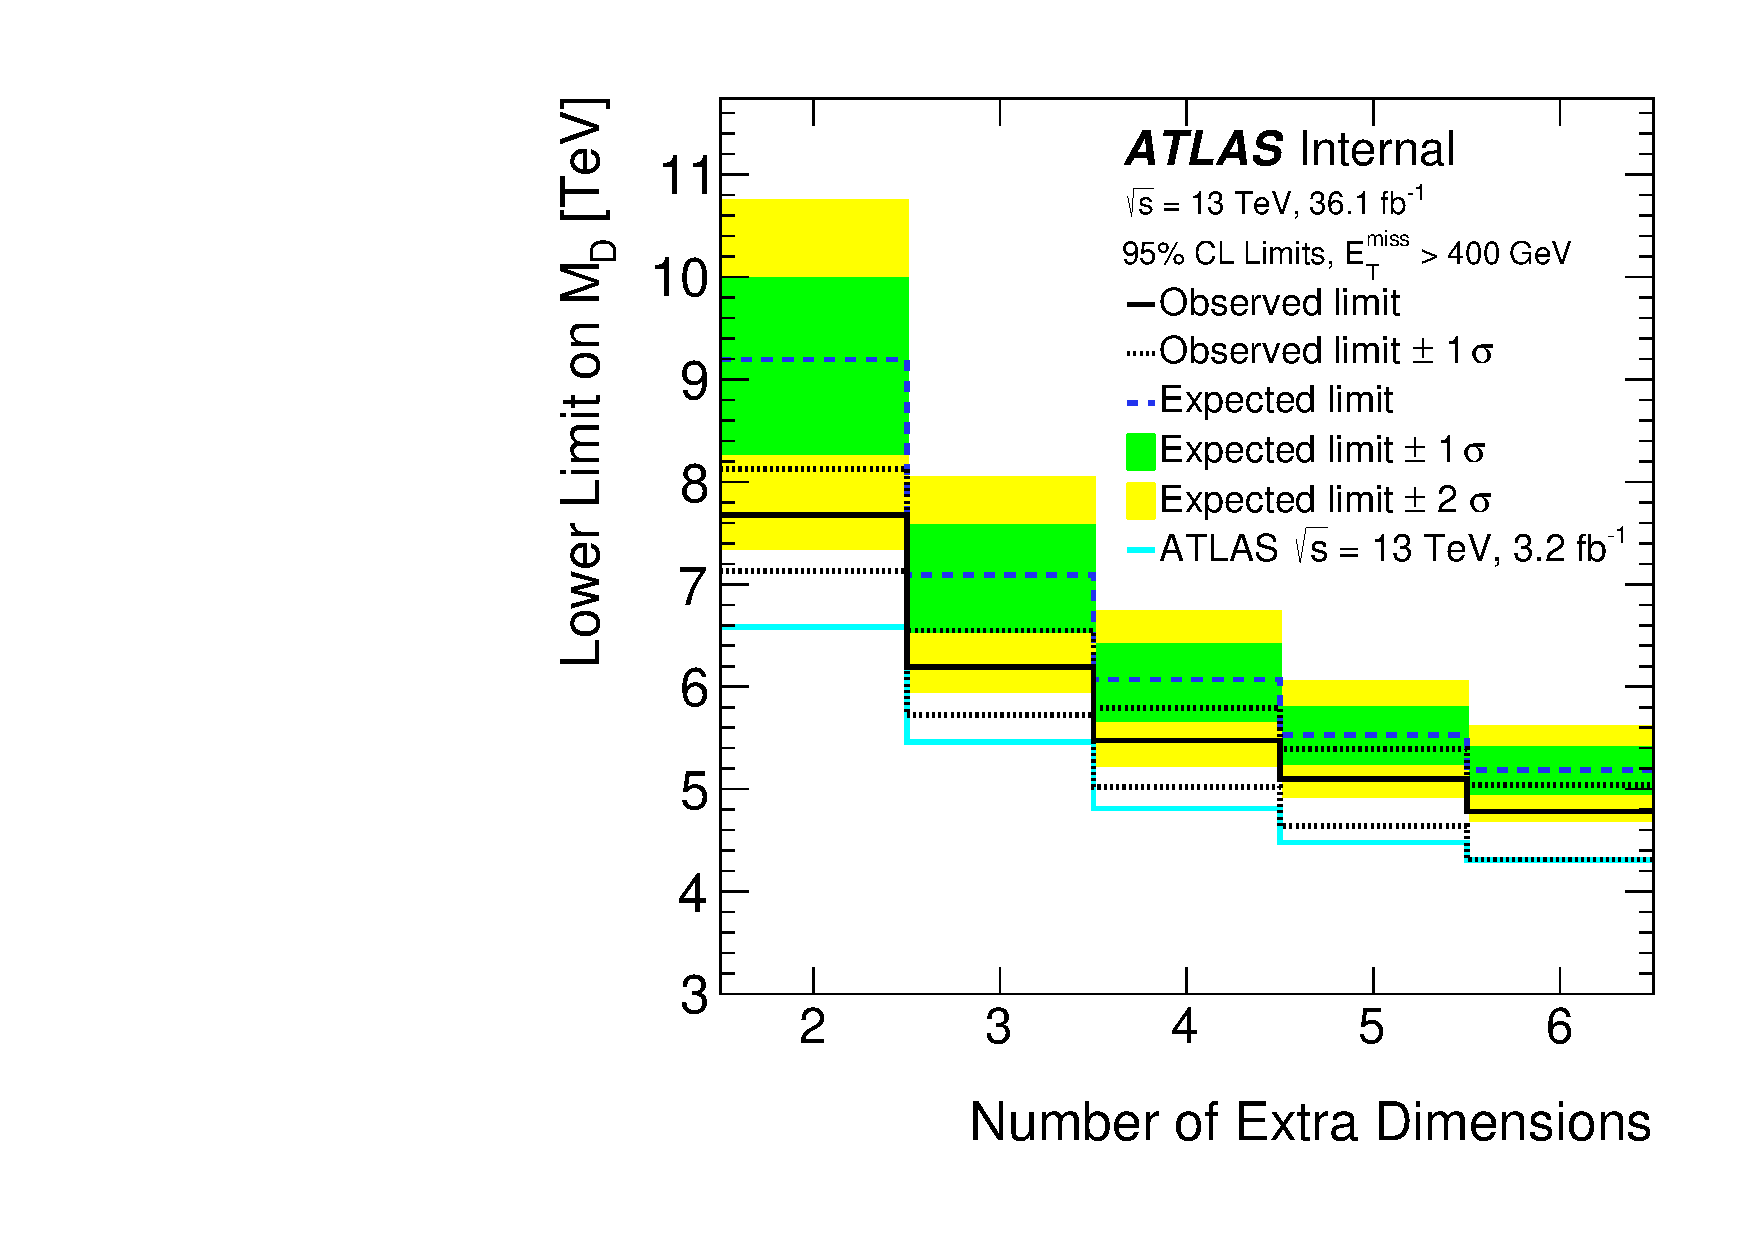
\includegraphics[width=10cm]{add_exclusion_observed}
  \caption{Expected and observed limits at 95\% CL on the fundamental Planck
    Scale in $4 + n$ dimensions, M$_\mathrm{\, D}$, as a function of the number
    of extra dimensions $n$. The dashed blue line shows the expected limit using
    $36.5~\ifb$, the green and yellow bands are the $\pm 1 \sigma$ and
    $\pm 2 \sigma$ uncertainties on the estimate. The solid black line is the
    observed limit while the cyan line represents the observed limits in the
    2015 analysis using $3.2~\ifb$.}
  \label{fig:add_observed}
\end{figure}
%%% Local Variables:
%%% mode: latex
%%% TeX-master: "../search_for_DM_LED_with_ATLAS"
%%% End:
